\documentclass[varwidth=true, border=2pt]{standalone}

\usepackage{pgfplots}
\usepackage{tikz}

\usetikzlibrary{calc,patterns,angles,quotes,spy}

\begin{document}
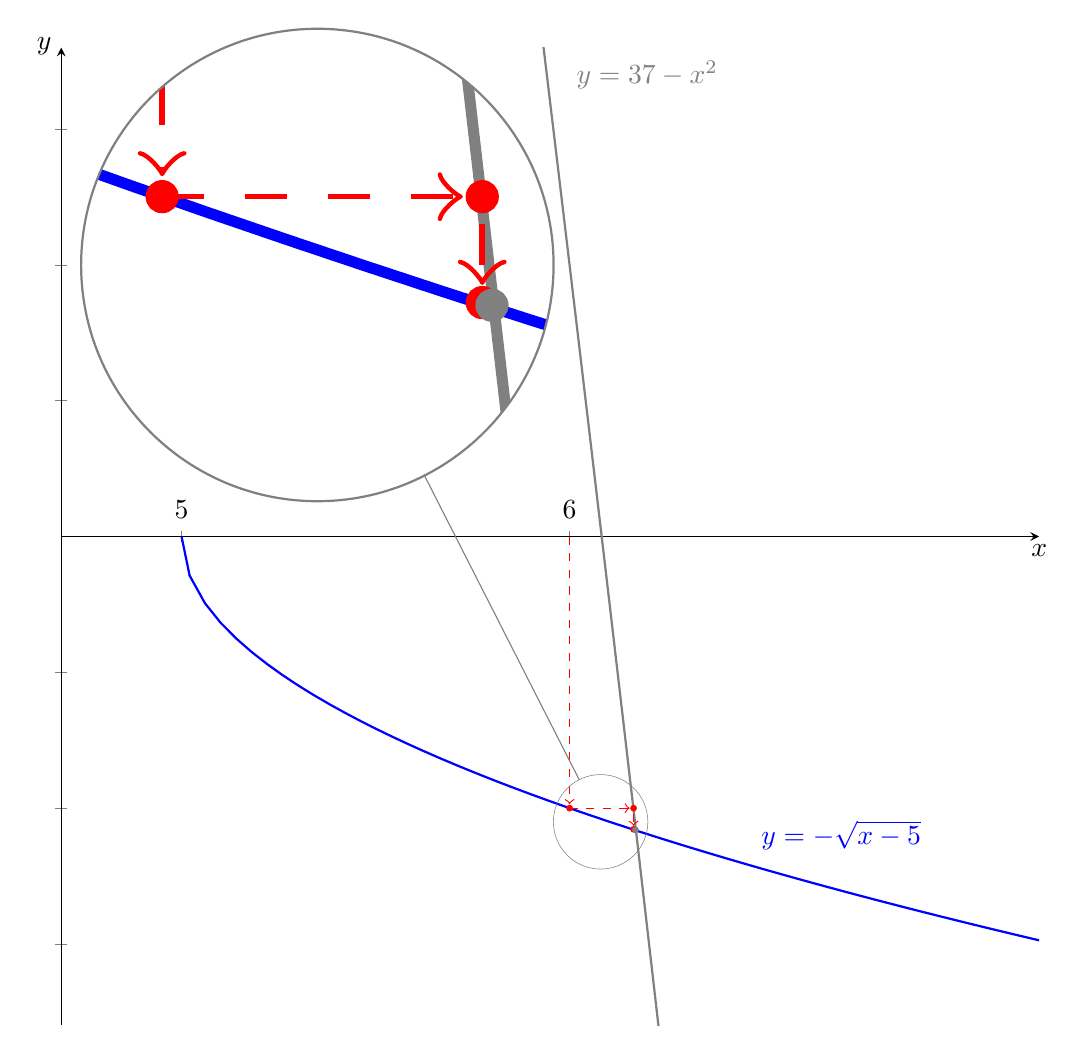
\begin{tikzpicture}[spy using outlines=
	{circle, magnification=5, connect spies}]
    \begin{axis}[
        legend pos=south east,
        axis x line=middle,
        axis y line=middle,
	every axis x label/.style={at={(current axis.right of origin)},anchor=north},
	every axis y label/.style={at={(current axis.above origin)},anchor=east},
	xtick={5, 6},
	xticklabels=\empty,
	yticklabels=\empty
        grid = none ,
        width=14cm,
        height=14cm,
        grid style={dashed, gray!1},
        xmin=4.9,     % start the diagram at this x-coordinate
        xmax= 7,    % end   the diagram at this x-coordinate
        ymin=-1.5,     % start the diagram at this y-coordinate
        ymax= 1.5,   % end   the diagram at this y-coordinate
        xlabel=$x$,
        ylabel=$y$,
        enlargelimits=true,
        tension=0.08]

        \addplot[domain=4.9:8,gray, thick,samples=250] {37-x^2}; % Parabola
        \addplot[domain=5:5.021, blue, thick,samples=250] {-6.9*(x-5};
         \addplot[domain=0:10, blue, thick,samples=250] {-sqrt(x-5)};
	
	\node[gray] (x0) at (axis cs: 6.2,1.7){$y = 37-x^2$};
	\node[blue] (y0) at (axis cs: 6.7,-1.1){$y = - \sqrt{x-5}$};
	
	\node (n5) at (axis cs:5,0.1){5};
	\node (n6) at (axis cs:6,0.1){6};

	
	\draw[red, dashed, ->](axis cs:6,0)--(axis cs:6, -0.985);
	\draw[red, dashed, ->](axis cs:6,-1)--(axis cs:6.155, -1);
	\draw[red, dashed, ->](axis cs:6.165,-1.02)--(axis cs:6.165, -1.065);

	\addplot[red, only marks, mark=*, mark size=1pt] coordinates {(6,-1)(6.165,-1)(6.165, -1.078)};
	\addplot[gray, only marks, mark=*, mark size=1pt] coordinates {(6.17,-1.08)};	
	
	\coordinate (spypoint) at (axis cs:6.08,-1.05);
	\coordinate (magnifyglass) at (axis cs:5.35,1);
	
	\spy [gray, size=6cm] on (spypoint) in node[fill=white] at (magnifyglass);
    \end{axis}
\end{tikzpicture}
\end{document}